%-------------------------------------------------------------------------------
% paper/cace/supplement.tex -- Supplementary material of the Computers &
% Chemical Engineering article (main.tex), revision 2 (2026-10-25).
% Asked for by the external review (points 3 and 8): the essential commands,
% the audit of the reference's sample files, and case C.
% Build: `make supplement.pdf` (the Makefile builds it with main.pdf).
% Every number here was read from the runs named in S1, on the tree of
% branch claude/c126-papers-revision (based on origin/main c11d0354a).
%-------------------------------------------------------------------------------
\documentclass[11pt]{article}
\usepackage[T1]{fontenc}
\usepackage[utf8]{inputenc}
\usepackage{lmodern}
\usepackage[english]{babel}
\usepackage[a4paper,margin=2.3cm]{geometry}
\usepackage{microtype}
\usepackage{booktabs}
\usepackage{tabularx}
\usepackage{array}
\usepackage{graphicx}
\usepackage{xcolor}
\usepackage{enumitem}
\usepackage{listings}
\usepackage[colorlinks=true,linkcolor=blue!50!black,urlcolor=blue!50!black]{hyperref}
\graphicspath{{figures/}{../whitepaper/figures/}}
\setlist{itemsep=2pt,topsep=3pt}
\newcommand{\code}[1]{\nolinkurl{#1}}
\makeatletter\g@addto@macro\UrlBreaks{\do\_\do\-}\makeatother
\renewcommand{\thesection}{S\arabic{section}}
\renewcommand{\thetable}{S\arabic{table}}
\renewcommand{\thefigure}{S\arabic{figure}}
\lstset{basicstyle=\ttfamily\footnotesize, columns=fullflexible,
        keepspaces=true, frame=single, rulecolor=\color{gray!50},
        breaklines=true, upquote=true}

\title{Supplementary material to ``Choupo: an open-source chemical process
simulator for education and research''}
\author{Vítor Geraldes, Pedro Mendes, Miguel Rodrigues}
\date{Revision 2 -- DRAFT}

\begin{document}
\maketitle

\section{Reproducing every number}
\label{s:repro}

All numbers in the article and in this supplement were produced on one
commit of the development line of \url{https://github.com/choupo-admin/choupo}
(the commit carrying this manuscript; based on \code{c11d0354a}).  With a
C++17 compiler and GNU make, from the repository root:

\begin{lstlisting}
make all -j3                         # the five binaries, no external library
./choupoSolve  <case>                # a steady case (application choupoSolve)
./choupoProps  <case>                # a property / fitting case (choupoProps)
python3 -I benchmarks/dwsim/compare.py all     # the five benchmark cases
python3 -I paper/cace/figures/gen_dspmde_fit.py    # data of Figure 4a
python3 -I paper/cace/figures/gen_sdem_traces.py   # data of Figure 4b
python3 -I bin/curate/check_mass_closure.py        # Table 3, mass column
python3 -I bin/curate/check_energy_closure.py      # Table 3, energy column
\end{lstlisting}

A case writes into its own directory, so each was copied to a scratch
directory before it was run.  Table~\ref{tab:repro} maps each item of the
article to its case and to the file it was read from.

\begin{table}[h]
\centering\footnotesize
\caption{Where each item of the article comes from.}
\label{tab:repro}
\begin{tabularx}{\linewidth}{>{\raggedright\arraybackslash}p{3.2cm}
                             >{\raggedright\arraybackslash}p{5.6cm}
                             >{\raggedright\arraybackslash}X}
\toprule
\textbf{item} & \textbf{case} & \textbf{read from} \\
\midrule
Listings 1--3 & \code{tutorials/steady/flash/flash01_benzene_toluene} &
  the run log; the refusal: the same case with \code{vaporFraction 0.3;}
  appended to \code{0/feed} \\
heater check (Sect.~3.2) & \code{tutorials/steady/heat/hx01_heater} &
  \code{converged/hotStream}; \code{reports/balances/globalEnergyBoundary.csv} \\
Figure 2 & \code{tutorials/props/curation/curate05_nrtl_acetone_methanol} &
  the CSV files the run writes (identical to
  \code{paper/whitepaper/data/}); $\chi^2$ from
  \code{heldout_residuals.csv} and the held-out dataset's \code{U95} \\
Figure 3, Table 4 & \code{tutorials/steady/flowsheets/cavett01_recycle_train}
  & the log (Newton history); \code{converged/P1};
  \code{reports/balances/*.csv}; Wegstein: \code{recycleSolver Wegstein;}
  in \code{system/solverDict} \\
Figure 4a & \code{tutorials/steady/membranes/membrane24_fit_then_simulate}
  (props mode) & \code{postProcessing/fit_NF270_FdL2021/rejections.csv};
  the fit's printed parameters and verdict \\
Figure 4b & probes built from
  \code{tutorials/steady/membranes/membrane12_sdem_nf270_nacl_traces} by
  \code{bin/curate/check_sdem.py}'s builder & \code{paper/cace/data/sdem_*.csv} \\
NanoFiltran comparison & \code{tutorials/props/membrane/nanofiltran_geraldesAlves2008}
  & \code{bin/curate/check_nanofiltran_reference.py} \\
electrodialysis & \code{tutorials/steady/electrodialysis/ed04_limiting_current_multiionic}
  & the printed \code{i_lim} of each unit; the measured values: the case's
  README (Table 4 of the source) \\
Tables 5--7 & \code{benchmarks/dwsim/<case>} & \code{compare.py}'s tables;
  each case's README \\
\bottomrule
\end{tabularx}
\end{table}

\section{The reference's stored states: what an audit of the sample files found}
\label{s:audit}

The comparison of the article is with the solved states stored in five
sample files of DWSIM, read at commit
\code{1abf72d1b6b41d3e9a8cc770d3cc4e8fc76e5766} of
\url{https://github.com/DanWBR/dwsim} (2026-07-17); the files record build
versions 8.8.0.0 (A, B, C), 6.5.2.0 (D) and 5.3.6858.20432 (E).  The
samples were not re-executed.  The findings below are facts about those
files, measured on their own numbers; they bound how finely each comparison
can resolve, and each is being offered to the program's maintainers.  None
of them is evidence about the quality of Choupo.

\begin{description}[leftmargin=1em]
\item[A (Cavett's problem)] The stored feed has 15 compounds and no
  $n$-undecane, and its total (5908.21~mol/s) matches neither reading of the
  primary specification's units; the primary's absolute pressures were
  entered as gauge pressures (800/270/49/13 + 14.7~psi); each of the three
  recycle blocks reports convergence after one iteration, and one passes on
  a state that differs from its source's (vapour fraction 0.38562 against
  0.38906, 20.39~kW apart); one separator stores its vapour and its liquid
  0.97~K apart; the stored state closes its first law to $+17.49$~kW.
\item[B (pressure-swing distillation)] The two bottoms specifications admit
  no steady state ($+0.14$~\% on the plant); the recycle stream carries
  1.47~\% more than the stream it copies, while its recycle block reports
  convergence after one iteration; the light distillate is stored 1.98~K
  below its own condenser stage; the property package lists the
  acetone--methanol NRTL interaction twice with different values.
\item[C (extraction with MIBK)] The column is adiabatic and cools by
  13.4~K (stages at 296.54, 295.81, 290.79 and 284.70~K); its first law on
  the stored enthalpies closes to $-0.54$~kW; two stored extractor
  specifications do not match their stored calculated values (in that mode
  they are not used); the package is a modified (Dortmund) UNIFAC.
\item[D (methanol from CO$_2$)] A 98.9~\% methanol distillate stored at
  184.69~K; two exchanger efficiencies stored above 100~\%; one adsorption
  constant carried as 3453.38 and 3454.38 in two rate expressions, and the
  kinetics depart from the article in three more places (an exponent of
  40\,000/RT for 36\,696, a rate constant at the lower bound of its
  interval, a parenthesis that moves a square root); a compressor with
  negative work; a stored plant flow balance of $-17.0$~\%; the hydrogen
  feed is stored two-phase at the compressor's suction.
\item[E (steam reforming)] The rates read partial pressures in atm where
  the article's are in bar; two of the three rates truncate the article's
  shared adsorption denominator; the third equilibrium constant is not the
  product of the first two (19.65 against 40.54 at 1000~K, bar basis); the
  stored duty, 1221.81~kW, is 2.6 times the heat of reaction of the stored
  conversion; the pre-exponential factors are rounded.
\end{description}

\section{Case C: acetone extraction with MIBK}
\label{s:caseC}

Choupo's predictive UNIFAC did not describe the water--MIBK miscibility
gap well enough (its water-rich branch sits at the flash's composition
floor, against 0.0038 measured), so a liquid--liquid NRTL set was curated
from the measured tie lines of Choi and Rhim (1986, J.\ Korean Inst.\ Chem.\
Eng.\ 24, 185--194), converted from the article's table by arithmetic only.
At the midpoints of the authors' calculated tie lines it returns those lines
to within 0.0035 mole fraction on lines 1--9 and 0.018 on line 10, nearest
the plait point; against the measured lines it misses the binary edge (water
in MIBK 0.013 against 0.118 measured), as the authors' own calculated line
does.  On the tree of this revision Choupo's four-stage extractor and the
same cascade written as four mixers and four flashes agree to every printed
digit: extract 984.05~mol/s, raffinate 293.29~mol/s, acetone recovery
1.0000, against the reference's stored 911.32, 366.01 and 0.9991.  The
UNIFAC variant refuses by name.  The two programs solve different problems
(adiabatic against isothermal), and temperature moves the split, so this
case is not used in the article's comparison.

\section{Case E: the grid study}
\label{s:grid}

Table~5 of the article gives Choupo's methane conversion against the number
of RK4 steps through the bed.  The case was first built with 400 steps; at
that resolution its outlet was 0.85~\% short of its own limit, and the case
now uses 25\,600 (0.4~s of computing).  Twenty steps -- the sample's stored
volume increment -- refuse by name in Choupo: the first step drives the
hydrogen partial pressure to zero and the rate law has no value there.  The
other benchmark with a bed, case D, was checked the same way: its methanol
product moves by $10^{-9}$ relative between 5000 and 20\,000 steps.

\section{The browser front-end}
\label{s:gui}

\begin{figure}[h]
\centering
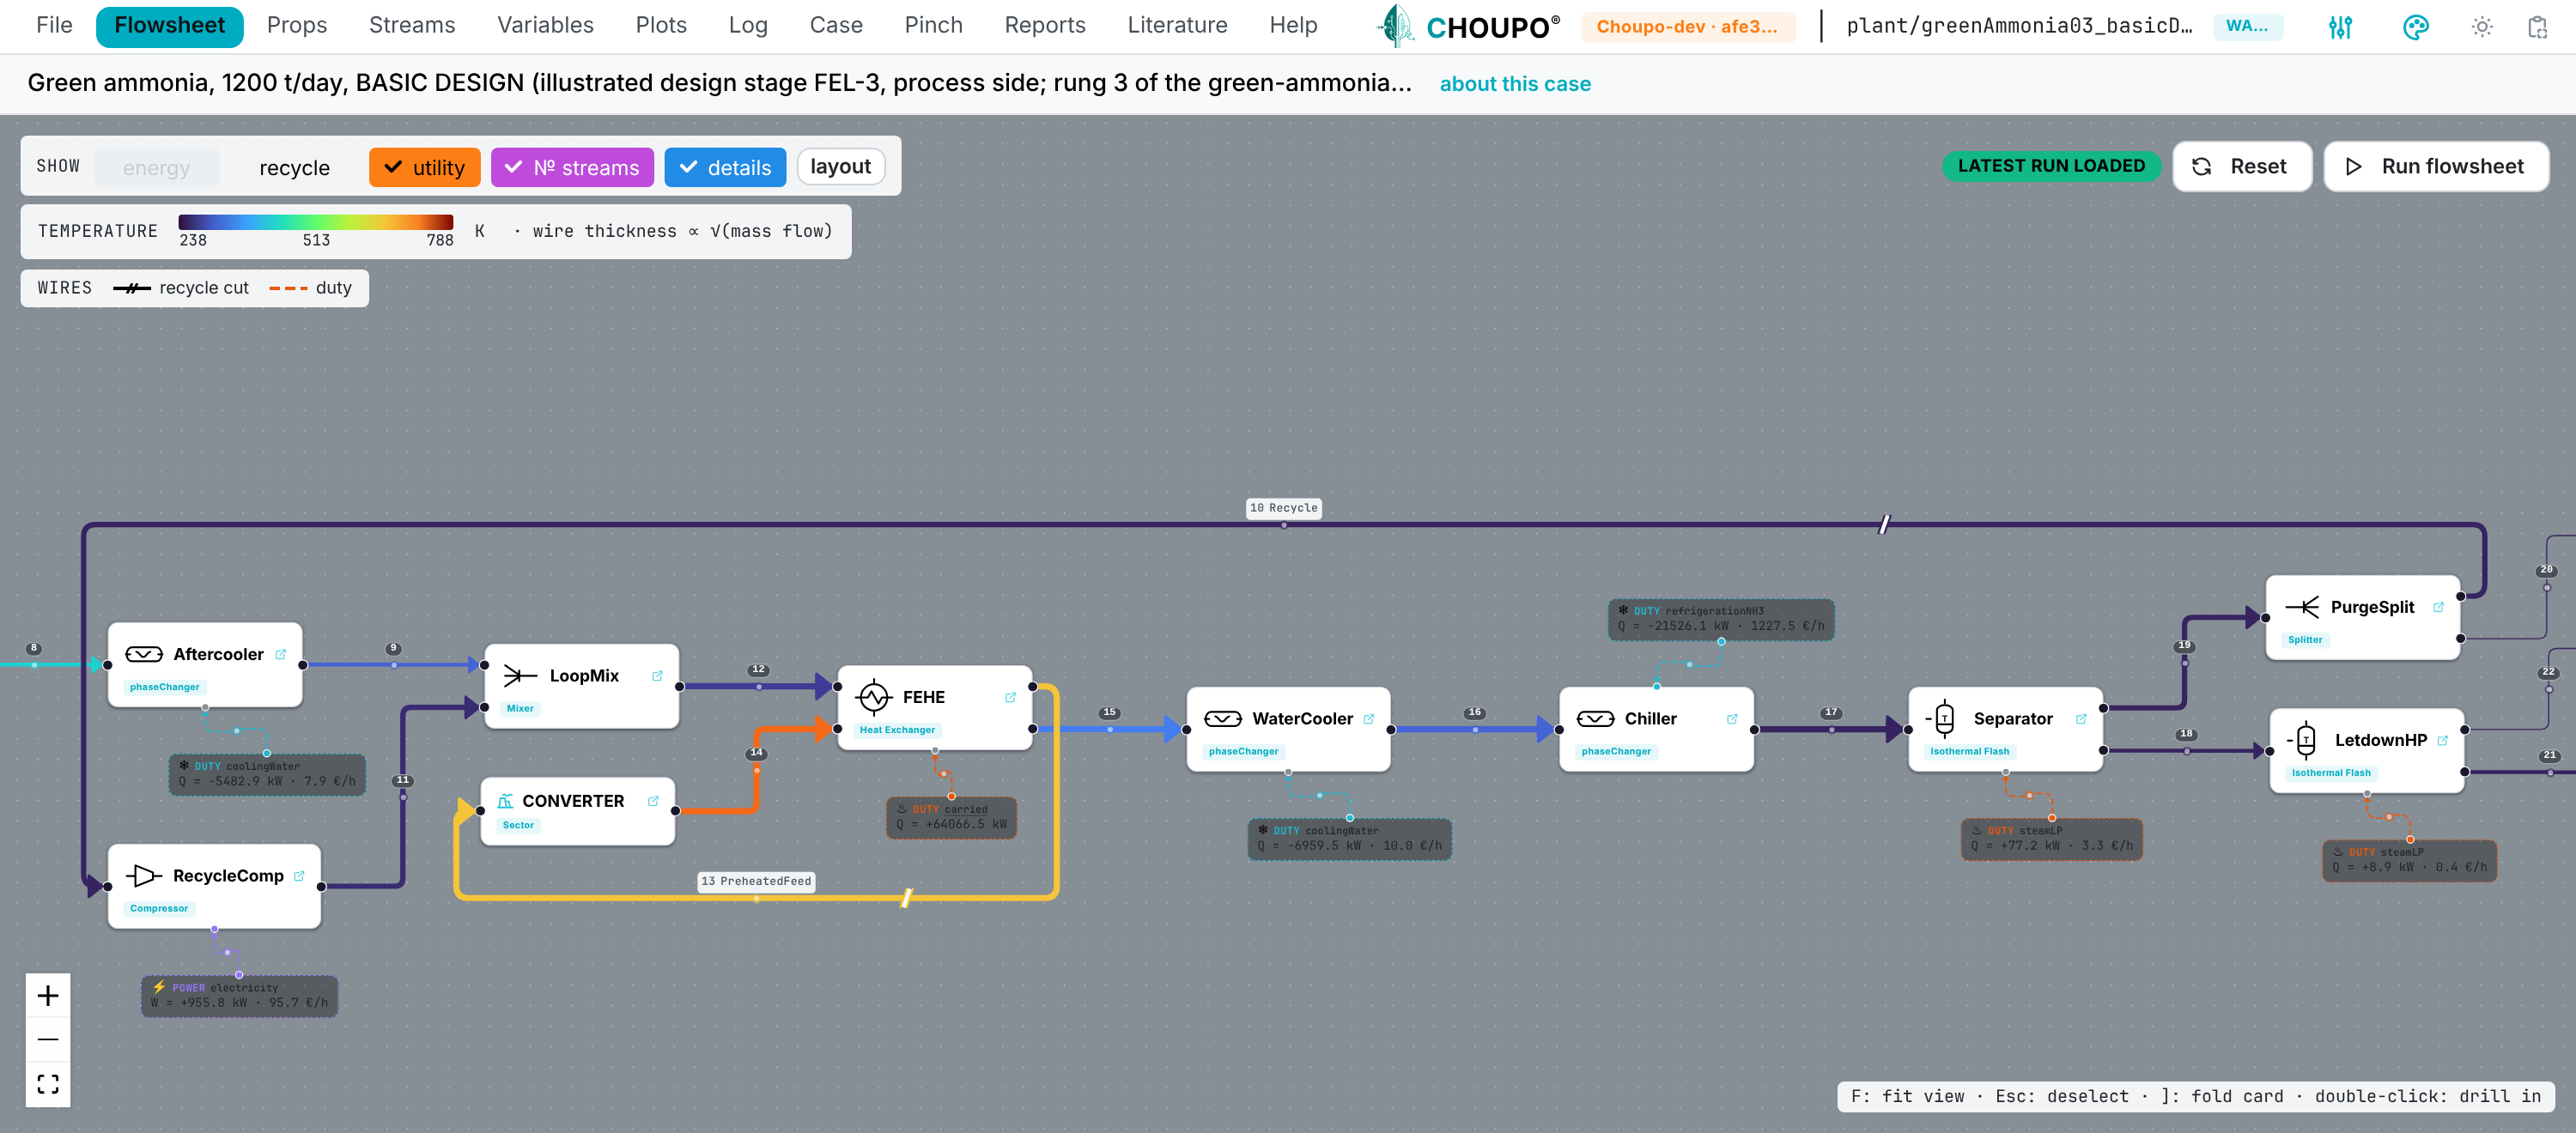
\includegraphics[width=\textwidth]{gui_flowsheet.png}
\caption{The browser front-end on \texttt{tutorials/plant/greenAmmonia03\_basicDesign},
run in the page by the WebAssembly build of the engine (captured
2026-10-21 by \texttt{paper/whitepaper/figures/capture\_gui.mjs}).  Streams are coloured
by the temperature the engine published; slashed wires are the recycle
tears; \texttt{CONVERTER} is a sector of three catalyst beds and two
inter-bed coolers.  Nothing on the screen is computed in the browser.}
\end{figure}

\begin{figure}[h]
\centering
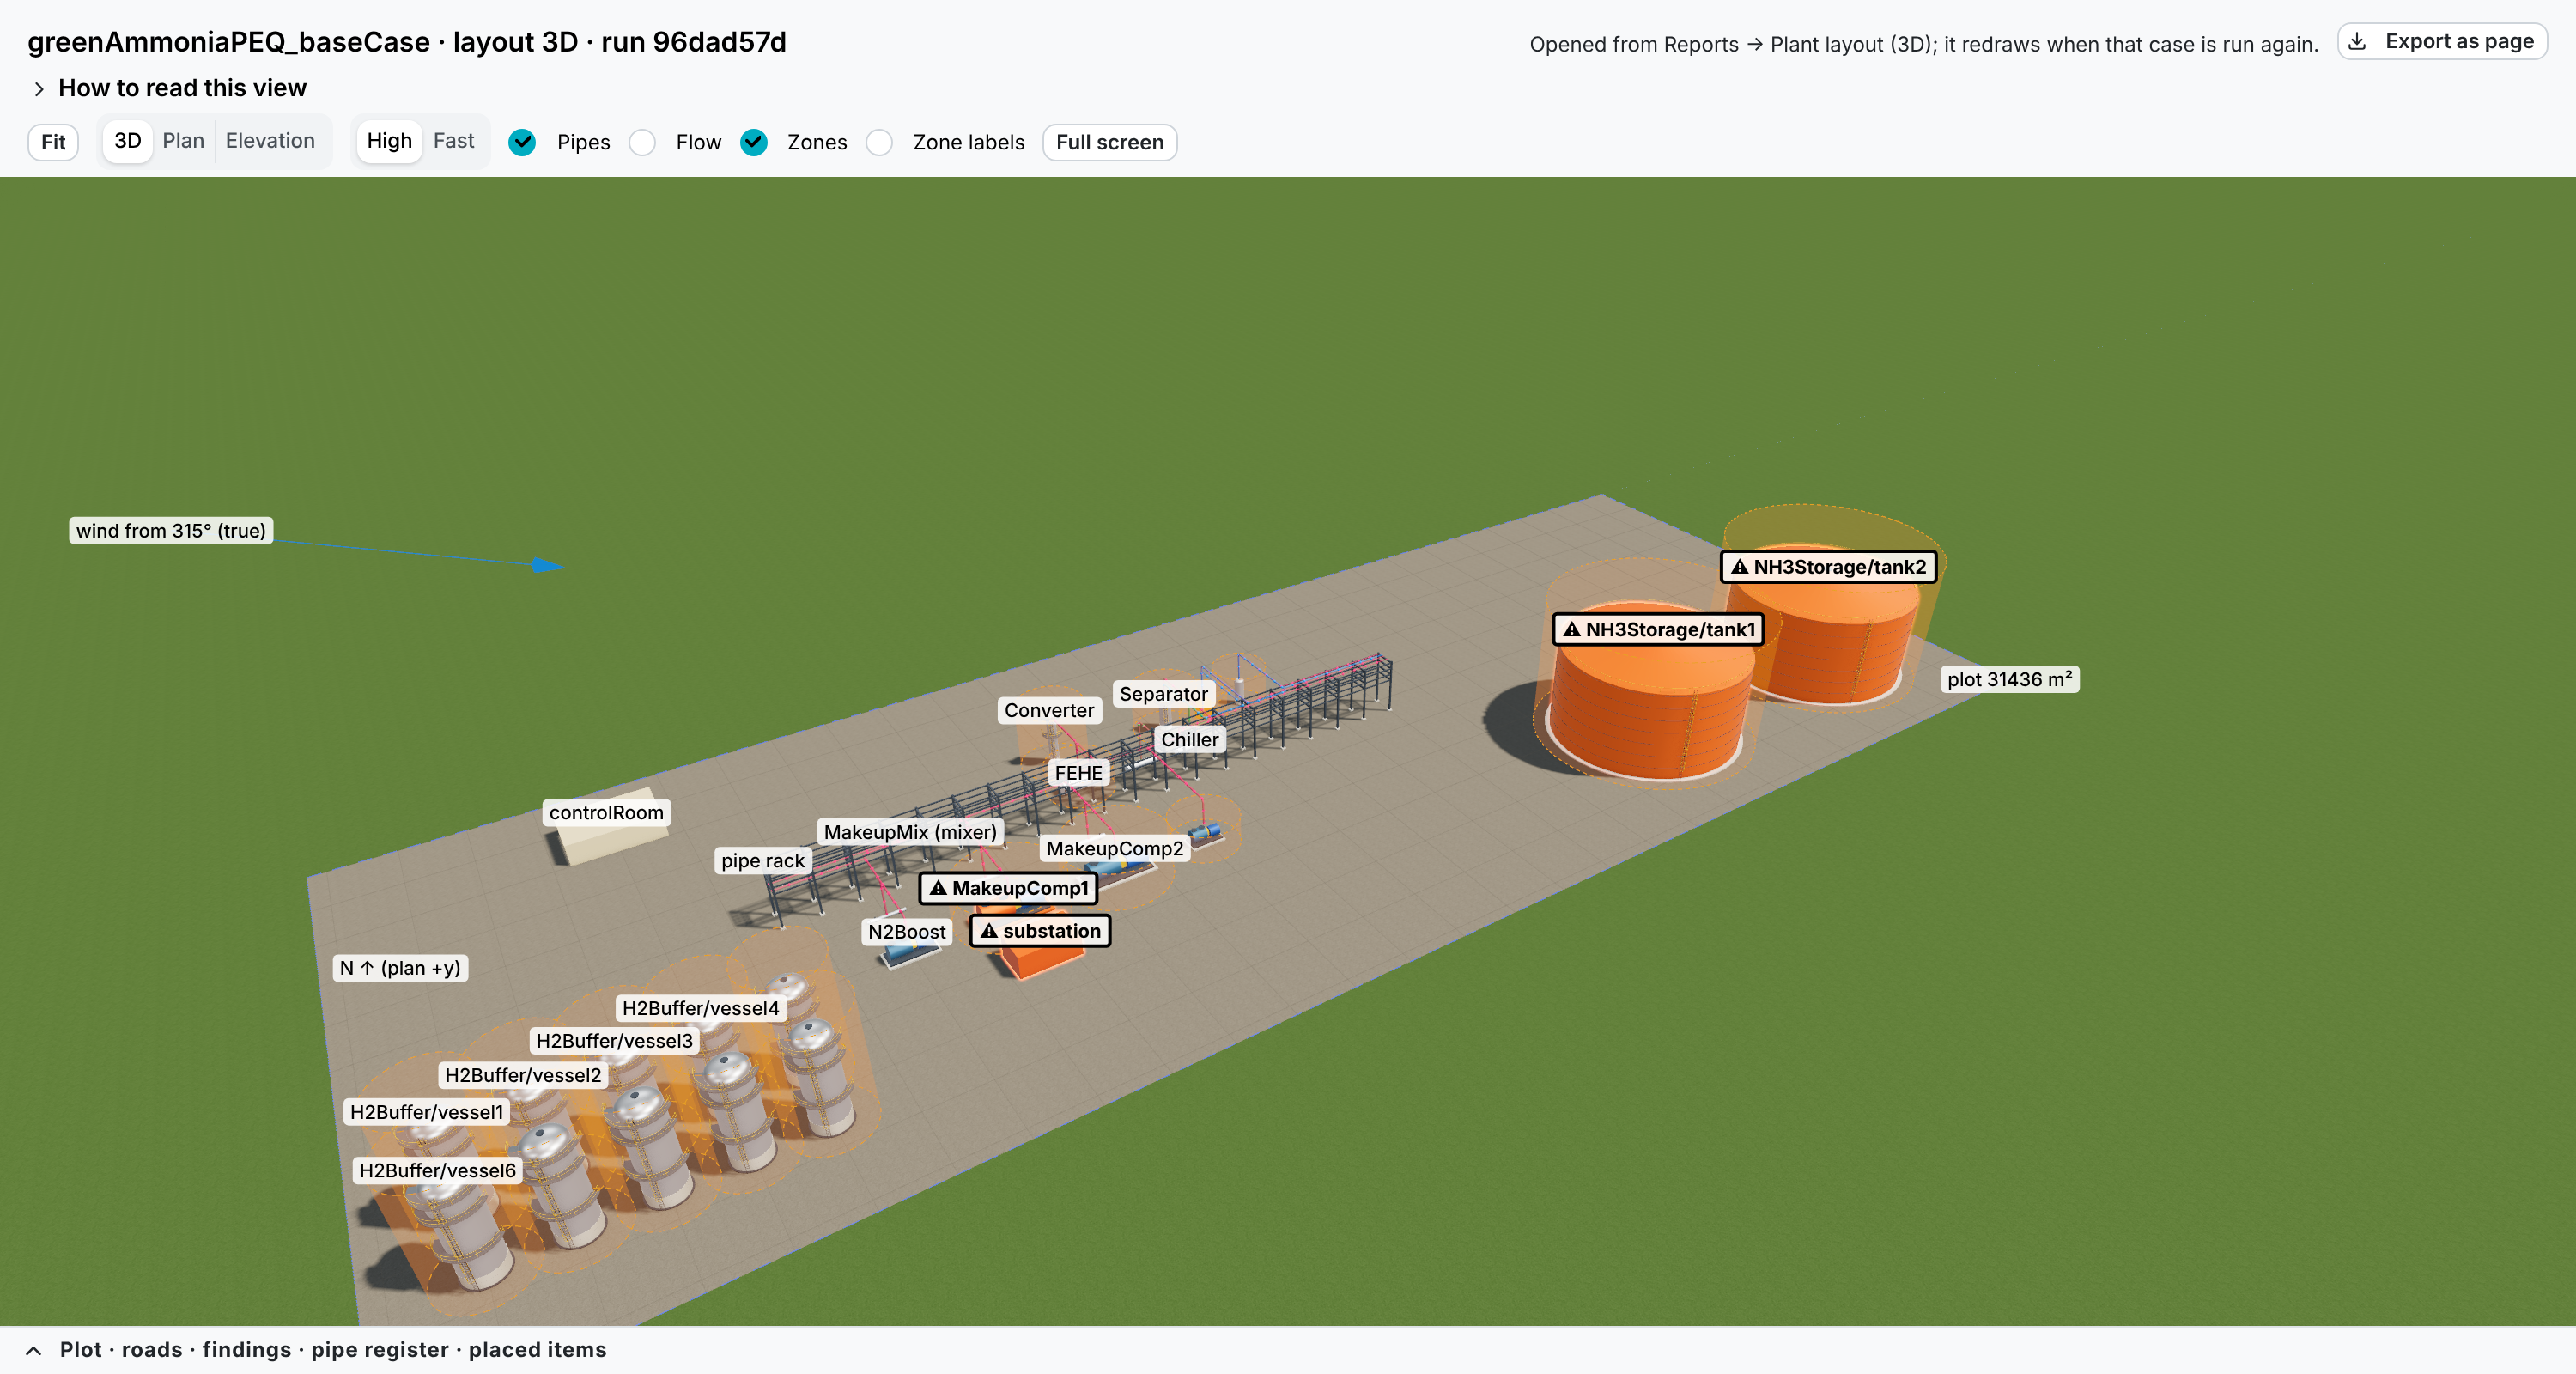
\includegraphics[width=\textwidth]{gui_layout3d.png}
\caption{The plot plan of \texttt{tutorials/plant/greenAmmoniaPEQ\_baseCase},
drawn from the layout block of the run's result: each item where the case
places it, on the envelope the sizing pass published, with the case's
declared hazardous-area zones and the pipes the engine routed.}
\end{figure}

\end{document}
